\documentclass[9pt]{extarticle}
\usepackage[a4paper,landscape,margin=1.2cm]{geometry}
\usepackage{booktabs,longtable,multirow,amsmath,graphicx,pdfpages,xcolor,caption}
\captionsetup{font=small,labelfont=bf}
\renewcommand{\arraystretch}{1.05}
\begin{document}
\begin{center}{\Large\bfseries Constant-Lagrangian inflow pipeline applied to SPARC (175 galaxies)}\\[4pt]
{\small Single-L and two-L models of de Haas (SPARC $H_z$ paper, Eqs.\ 17--18 and 24--26), $H_z=2.2\times10^{-18}\,\mathrm{s^{-1}}$ fixed; fits on $v^2(r)$ with $\sigma_{v^2}=2V_\mathrm{obs}\delta V_\mathrm{obs}$; data Lelli, McGaugh \& Schombert (2016).}\end{center}
\section*{Pipeline}
\begin{enumerate}\itemsep0pt
\item Single-L fit $(R,M)$ to every galaxy (14 starting radii, bounded least squares).
\item Wave screen on the weighted residuals $\mathrm{WR}_i=(v^2_\mathrm{obs}-v^2_\mathrm{mod})/\sigma_{v^2}$: one-sided Wald--Wolfowitz runs test ($p_\mathrm{runs}$, too few sign runs) and the best agreement $A_{+-+}$ ($A_{-+-}$) of the residual signs with a three-segment template (each segment $\geq2$ points). Categories: \textbf{A} adequate ($p_\mathrm{runs}\ge0.05$, $\chi^2_\nu\le1$); \textbf{B} $+-+$ wave ($p_\mathrm{runs}<0.05$, $A_{+-+}\ge0.8$, $A_{+-+}>A_{-+-}$); \textbf{C} $-+-$ wave (same with signs reversed); \textbf{D} structured, other ($p_\mathrm{runs}<0.05$); \textbf{E} poor, unstructured ($p_\mathrm{runs}\ge0.05$, $\chi^2_\nu>1$).
\item Category B: two-L fit seeded at $R_2\simeq r_{\times1}/0.8$ ($r_{\times1}$ = first $+\to-$ crossover), cross-checked with a global grid search; also two-L\,+\,$\Phi_\mathrm{BH}$.
\item Accept the two-L description when $\Delta\mathrm{BIC}=\mathrm{BIC}_\mathrm{2L}-\mathrm{BIC}_\mathrm{1L}<-6$.
\item Accepted fits with $n\le13$ are marked tentative.
\end{enumerate}
Post-hoc flags on accepted fits (not part of the acceptance rule): \textbf{N} = not a nested configuration ($M_2<M_1$, or $v^2$ drops by more than 40\% at $R_2$); \textbf{M} = still inadequate after two-L ($\chi^2_\nu>2$), i.e.\ more regions (virial windows, a third Lagrangian) needed.

\begin{table}[h]\centering\small\caption{Pipeline outcome.}\begin{tabular}{lr}\toprule Category after single-L fit & $N$\\\midrule
A: single-L adequate & 54\\
B: $+-+$ wave (double-L candidate) & 45\\
C: $-+-$ wave (declining / virial) & 41\\
D: structured, other & 18\\
E: poor, unstructured & 17\\
\midrule
B: two-L accepted ($\Delta$BIC$<-6$) & 23\\ \quad of which tentative ($n\le13$) & 5\\ \quad of which flagged N (not nested) & 5\\ \quad of which flagged M (still $\chi^2_\nu>2$) & 8\\
B: single-L kept ($\Delta$BIC$\ge-6$) & 22\\
2018 RMWRSS double-fit galaxies recovered as accepted two-L & 8 / 13\\
Seeded two-L start reached the global-grid optimum & 31 / 45\\
\bottomrule\end{tabular}\end{table}\clearpage
{\scriptsize\setlength{\tabcolsep}{3.5pt}
\begin{longtable}{lllrrrrrrrrcrl}
\caption{Single-L fit and wave screen for all 175 SPARC galaxies, sorted by category and $\chi^2_\nu$. $R$ in kpc, $M$ in $10^9M_\odot$; $\dagger$ = 2018 RMWRSS double-fit galaxy.}\\\toprule
Galaxy & Type & Q & $n$ & $R$ & $M$ & $\chi^2_\nu$ & RMS$_\mathrm{rel}$ & $p_\mathrm{runs}$ & $A_{+-+}$ & $A_{-+-}$ & Cat & $\Delta$BIC & Outcome\\\midrule\endfirsthead
\toprule Galaxy & Type & Q & $n$ & $R$ & $M$ & $\chi^2_\nu$ & RMS$_\mathrm{rel}$ & $p_\mathrm{runs}$ & $A_{+-+}$ & $A_{-+-}$ & Cat & $\Delta$BIC & Outcome\\\midrule\endhead
\bottomrule\endfoot
UGC09992 & Im & 2 & 5 & $0.431\pm0.4$ & $0.0414\pm0.047$ & 0.00 & 0.018 & 1.000 & -- & -- & A & -- & \\
UGC06628 & Sm & 2 & 7 & $1.05\pm0.41$ & $0.165\pm0.088$ & 0.00 & 0.025 & 0.113 & 0.29 & 0.86 & A & -- & \\
F561--1 & Sm & 3 & 6 & $2.22\pm0.74$ & $0.524\pm0.25$ & 0.01 & 0.021 & 0.500 & 0.50 & 0.50 & A & -- & \\
UGC05999 & Im & 2 & 5 & $4.83\pm0.59$ & $4.62\pm0.9$ & 0.02 & 0.013 & 1.000 & -- & -- & A & -- & \\
NGC3949 & Sbc & 2 & 7 & $1.34\pm0.17$ & $3.27\pm0.6$ & 0.03 & 0.019 & 0.358 & 0.86 & 0.29 & A & -- & \\
F563--V2 & Im & 1 & 10 & $1.83\pm0.24$ & $2.33\pm0.53$ & 0.03 & 0.048 & 0.163 & 0.50 & 0.90 & A & -- & \\
F574--2 & Sm & 3 & 5 & $5.57\pm3.1$ & $1.01\pm1.1$ & 0.03 & 0.143 & 1.000 & -- & -- & A & -- & \\
UGC05750 & Sdm & 1 & 11 & $4.78\pm0.58$ & $2.8\pm0.79$ & 0.04 & 0.065 & 0.225 & 0.82 & 0.64 & A & -- & \\
F571--V1 & Sd & 2 & 7 & $3.54\pm0.76$ & $2.38\pm0.74$ & 0.04 & 0.060 & 0.358 & 0.71 & 0.57 & A & -- & \\
CamB & Im & 2 & 9 & $1.37\pm0.28$ & $0.0865\pm0.048$ & 0.04 & 0.044 & 0.500 & 0.67 & 0.78 & A & -- & \\
F565--V2 & Im & 2 & 7 & $3.56\pm0.61$ & $2.5\pm0.74$ & 0.04 & 0.085 & 0.113 & 0.86 & 0.29 & A & -- & \\
UGC08837 & Im & 2 & 8 & $2.77\pm0.31$ & $0.915\pm0.26$ & 0.05 & 0.041 & 0.223 & 0.88 & 0.50 & A & -- & \\
UGC07577 & Im & 2 & 9 & $1.23\pm0.53$ & $0.0556\pm0.061$ & 0.06 & 0.272 & 0.051 & 0.89 & 0.67 & A & -- & \\
D512--2 & Im & 2 & 4 & $0.997\pm0.16$ & $0.132\pm0.041$ & 0.07 & 0.055 & 1.000 & -- & -- & A & -- & \\
UGC10310 & Sm & 1 & 7 & $1.58\pm0.25$ & $0.758\pm0.18$ & 0.07 & 0.049 & 0.560 & 0.43 & 0.71 & A & -- & \\
UGC02023 & Im & 2 & 5 & $2.97\pm1.4$ & $1.66\pm2$ & 0.08 & 0.172 & 1.000 & -- & -- & A & -- & \\
NGC4068 & Im & 2 & 6 & $1.44\pm0.21$ & $0.297\pm0.1$ & 0.08 & 0.077 & 0.819 & 0.50 & 0.50 & A & -- & \\
UGC07261 & Sdm & 2 & 7 & $0.922\pm0.14$ & $0.431\pm0.09$ & 0.09 & 0.041 & 0.113 & 0.86 & 0.43 & A & -- & \\
UGC06930 & Sd & 1 & 10 & $2.19\pm0.34$ & $2.19\pm0.43$ & 0.10 & 0.044 & 0.103 & 0.70 & 0.90 & A & -- & \\
UGC07559 & Im & 2 & 7 & $1.05\pm0.19$ & $0.115\pm0.04$ & 0.11 & 0.152 & 0.181 & 1.00 & 0.29 & A & -- & \\
NGC4085 & Sc & 2 & 7 & $1.9\pm0.15$ & $3.49\pm0.46$ & 0.13 & 0.038 & 0.560 & 0.43 & 0.71 & A & -- & \\
F563--V1 & Im & 3 & 6 & $1.98\pm0.77$ & $0.159\pm0.096$ & 0.14 & 0.110 & 0.240 & 0.00 & 1.00 & A & -- & \\
F567--2 & Sm & 3 & 5 & $2.17\pm0.67$ & $0.527\pm0.25$ & 0.15 & 0.089 & 1.000 & -- & -- & A & -- & \\
NGC3877 & Sc & 2 & 13 & $2.27\pm0.17$ & $6.15\pm0.61$ & 0.15 & 0.062 & 0.076 & 0.46 & 0.92 & A & -- & \\
D564--8 & Im & 2 & 6 & $1.07\pm0.13$ & $0.0647\pm0.015$ & 0.15 & 0.092 & 0.181 & 0.83 & 0.17 & A & -- & \\
UGC07608 & Im & 1 & 8 & $1.8\pm0.31$ & $0.809\pm0.26$ & 0.16 & 0.092 & 0.223 & 0.88 & 0.50 & A & -- & \\
UGC04483 & Im & 2 & 8 & $0.344\pm0.049$ & $0.0189\pm0.0042$ & 0.17 & 0.188 & 0.582 & 0.88 & 0.38 & A & -- & \\
UGC11557 & Sdm & 2 & 12 & $3.2\pm0.42$ & $2.26\pm0.52$ & 0.18 & 0.308 & 0.179 & 0.58 & 0.83 & A & -- & \\
UGC05918 & Im & 2 & 8 & $1.08\pm0.18$ & $0.18\pm0.047$ & 0.19 & 0.129 & 0.063 & 0.88 & 0.50 & A & -- & \\
UGC05005 & Im & 1 & 11 & $5.97\pm0.72$ & $5.36\pm1.2$ & 0.19 & 0.278 & 0.074 & 0.91 & 0.55 & A & -- & \\
UGC07866 & Im & 2 & 7 & $0.671\pm0.16$ & $0.0598\pm0.024$ & 0.21 & 0.170 & 0.113 & 1.00 & 0.14 & A & -- & \\
F583--1 & Sm & 1 & 25 & $2.92\pm0.19$ & $1.78\pm0.22$ & 0.21 & 0.250 & 0.059 & 0.88 & 0.64 & A & -- & \\
UGC06399 & Sm & 1 & 9 & $2.28\pm0.27$ & $1.64\pm0.3$ & 0.22 & 0.111 & 0.051 & 1.00 & 0.56 & A & -- & \\
UGCA281 & BCD & 3 & 7 & $0.335\pm0.037$ & $0.0281\pm0.0055$ & 0.29 & 0.186 & 0.736 & 0.86 & 0.43 & A & -- & \\
UGC04499 & Sdm & 1 & 9 & $1.89\pm0.14$ & $0.935\pm0.1$ & 0.35 & 0.100 & 0.051 & 1.00 & 0.56 & A & -- & \\
UGC06973 & Sab & 3 & 9 & $0.157\pm0.2$ & $0.373\pm0.49$ & 0.36 & 0.036 & 0.051 & 1.00 & 0.56 & A & -- & \\
NGC3917 & Scd & 1 & 17 & $3.09\pm0.13$ & $5.51\pm0.35$ & 0.40 & 0.040 & 0.165 & 0.59 & 0.88 & A & -- & \\
UGC04325 & Sm & 1 & 8 & $1.01\pm0.074$ & $0.778\pm0.08$ & 0.41 & 0.049 & 0.500 & 0.50 & 0.75 & A & -- & \\
UGC07151 & Scd & 1 & 11 & $1.02\pm0.061$ & $0.483\pm0.043$ & 0.45 & 0.070 & 0.225 & 0.91 & 0.55 & A & -- & \\
UGC07603 & Sd & 1 & 12 & $0.871\pm0.067$ & $0.317\pm0.036$ & 0.46 & 0.126 & 0.113 & 0.75 & 0.75 & A & -- & \\
DDO170 & Im & 2 & 8 & $2.92\pm0.15$ & $1.02\pm0.075$ & 0.50 & 0.076 & 0.937 & 0.62 & 0.62 & A & -- & \\
NGC3953 & Sbc & 1 & 8 & $2.12\pm0.3$ & $9.34\pm1.6$ & 0.52 & 0.048 & 0.075 & 0.38 & 1.00 & A & -- & \\
F583--4$^\dagger$ & Sc & 1 & 12 & $1.36\pm0.17$ & $0.487\pm0.085$ & 0.56 & 0.239 & 0.126 & 0.92 & 0.50 & A & -- & \\
NGC6789 & BCD & 2 & 4 & $0.41\pm0.12$ & $0.159\pm0.11$ & 0.58 & 0.258 & 1.000 & -- & -- & A & -- & \\
UGC07690 & Im & 2 & 7 & $0.349\pm0.11$ & $0.101\pm0.039$ & 0.66 & 0.103 & 0.113 & 0.43 & 0.86 & A & -- & \\
UGC02259 & Sdm & 2 & 8 & $0.98\pm0.073$ & $0.625\pm0.057$ & 0.66 & 0.052 & 0.582 & 0.88 & 0.38 & A & -- & \\
UGC06818 & Sm & 2 & 8 & $3.77\pm0.45$ & $2.58\pm0.7$ & 0.68 & 0.274 & 0.223 & 0.75 & 0.75 & A & -- & \\
UGC07089 & Sdm & 2 & 12 & $2.83\pm0.27$ & $1.49\pm0.25$ & 0.70 & 0.199 & 0.113 & 0.92 & 0.58 & A & -- & \\
UGC07232 & Im & 2 & 4 & $0.504\pm0.11$ & $0.12\pm0.057$ & 0.71 & 0.186 & 1.000 & -- & -- & A & -- & \\
UGC06923 & Im & 2 & 6 & $1.82\pm0.27$ & $1.25\pm0.3$ & 0.71 & 0.226 & 0.500 & 0.17 & 0.83 & A & -- & \\
UGC06667 & Scd & 1 & 9 & $2.25\pm0.15$ & $1.58\pm0.17$ & 0.72 & 0.145 & 0.110 & 1.00 & 0.56 & A & -- & \\
UGC06917 & Sm & 1 & 11 & $2.15\pm0.14$ & $2.18\pm0.21$ & 0.74 & 0.086 & 0.175 & 0.82 & 0.55 & A & -- & \\
NGC4389 & Sbc & 3 & 6 & $2.83\pm0.39$ & $3.63\pm1.1$ & 0.75 & 0.176 & 0.181 & 0.83 & 0.17 & A & -- & \\
UGC05414 & Im & 1 & 6 & $1.57\pm0.14$ & $0.567\pm0.088$ & 0.93 & 0.137 & 0.181 & 0.83 & 0.17 & A & -- & \\
\midrule
F568--1 & Sc & 1 & 12 & $2.67\pm0.32$ & $4.29\pm0.81$ & 0.05 & 0.094 & 0.008 & 1.00 & 0.50 & B & 4.6 & single-L kept\\
F579--V1 & Sc & 1 & 14 & $0.983\pm0.23$ & $1\pm0.29$ & 0.10 & 0.108 & 0.003 & 0.93 & 0.79 & B & 4.5 & single-L kept\\
UGC08286 & Scd & 1 & 17 & $1.12\pm0.061$ & $0.667\pm0.046$ & 0.15 & 0.028 & 0.019 & 0.94 & 0.71 & B & 5.5 & single-L kept\\
F574--1 & Sd & 1 & 14 & $2.31\pm0.16$ & $1.99\pm0.2$ & 0.16 & 0.109 & 0.003 & 1.00 & 0.71 & B & 3.7 & single-L kept\\
KK98--251 & Im & 2 & 15 & $1.55\pm0.11$ & $0.228\pm0.038$ & 0.18 & 0.066 & 0.013 & 0.93 & 0.60 & B & 4.6 & single-L kept\\
F568--3 & Sd & 1 & 18 & $3.65\pm0.24$ & $3.86\pm0.54$ & 0.19 & 0.092 & 0.014 & 0.94 & 0.72 & B & 4.0 & single-L kept\\
NGC5005 & Sbc & 1 & 18 & $0.397\pm0.13$ & $2.11\pm0.77$ & 0.20 & 0.087 & 0.001 & 1.00 & 0.78 & B & 4.8 & single-L kept\\
UGCA444 & Im & 2 & 36 & $0.759\pm0.074$ & $0.0805\pm0.014$ & 0.26 & 0.223 & 7.6e-06 & 0.97 & 0.64 & B & 1.2 & single-L kept\\
UGC12632 & Sm & 1 & 15 & $2.18\pm0.15$ & $1.02\pm0.1$ & 0.28 & 0.179 & 0.002 & 1.00 & 0.60 & B & 3.7 & single-L kept\\
NGC0100 & Scd & 1 & 21 & $2.27\pm0.14$ & $1.56\pm0.16$ & 0.37 & 0.146 & 0.002 & 0.90 & 0.57 & B & 0.2 & single-L kept\\
NGC2976 & Sc & 2 & 27 & $1.24\pm0.056$ & $1.21\pm0.14$ & 0.47 & 0.155 & 0.013 & 0.85 & 0.74 & B & 1.1 & single-L kept\\
NGC4214 & Im & 2 & 14 & $0.188\pm0.041$ & $0.09\pm0.022$ & 0.53 & 0.122 & 0.010 & 0.93 & 0.79 & B & -0.6 & single-L kept\\
UGC06446$^\dagger$ & Sd & 1 & 17 & $1.22\pm0.14$ & $0.679\pm0.098$ & 0.67 & 0.147 & 0.004 & 0.94 & 0.82 & B & -2.9 & single-L kept\\
UGC08550 & Sd & 1 & 11 & $0.685\pm0.057$ & $0.179\pm0.019$ & 0.68 & 0.061 & 0.013 & 1.00 & 0.64 & B & 2.9 & single-L kept\\
NGC3109$^\dagger$ & Sm & 1 & 25 & $2.26\pm0.075$ & $0.942\pm0.061$ & 0.78 & 0.127 & 2.6e-04 & 0.96 & 0.68 & B & -5.9 & single-L kept\\
UGC05829$^\dagger$ & Im & 2 & 11 & $2.97\pm0.38$ & $1.32\pm0.32$ & 0.83 & 0.286 & 0.013 & 1.00 & 0.64 & B & -1.8 & single-L kept\\
NGC0055 & Sm & 2 & 21 & $3.14\pm0.1$ & $2.12\pm0.12$ & 1.04 & 0.135 & 1.3e-04 & 1.00 & 0.76 & B & -8.1 & two-L\\
UGC07524 & Sm & 1 & 31 & $2.78\pm0.1$ & $1.67\pm0.1$ & 1.07 & 0.249 & 6.7e-05 & 0.94 & 0.71 & B & -16.6 & two-L\\
ESO079--G014 & Sbc & 1 & 15 & $5.09\pm0.18$ & $15.9\pm0.84$ & 1.12 & 0.345 & 0.009 & 0.93 & 0.67 & B & -1.2 & single-L kept\\
UGC07125 & Sm & 1 & 13 & $2.94\pm0.24$ & $1.07\pm0.12$ & 1.15 & 0.150 & 0.007 & 1.00 & 0.69 & B & -5.4 & single-L kept\\
UGC07399 & Sdm & 1 & 10 & $0.852\pm0.059$ & $0.7\pm0.066$ & 1.29 & 0.098 & 0.025 & 0.90 & 0.70 & B & -3.1 & single-L kept\\
D631--7$^\dagger$ & Im & 1 & 16 & $2.44\pm0.13$ & $0.79\pm0.08$ & 1.33 & 0.184 & 0.002 & 1.00 & 0.56 & B & -10.4 & two-L\\
NGC3972$^\dagger$ & Sbc & 1 & 10 & $2.14\pm0.16$ & $3.28\pm0.38$ & 1.42 & 0.138 & 0.022 & 1.00 & 0.50 & B & -5.5 & single-L kept\\
UGC06614 & Sa & 1 & 13 & $1.69\pm0.87$ & $4.6\pm2.6$ & 1.62 & 0.158 & 0.005 & 0.92 & 0.77 & B & -9.8 & two-L (tent.) [N]\\
UGC07323 & Sdm & 1 & 10 & $2.62\pm0.2$ & $2.03\pm0.31$ & 1.68 & 0.284 & 0.036 & 1.00 & 0.50 & B & -5.6 & single-L kept\\
NGC4010 & Sd & 2 & 12 & $3.28\pm0.22$ & $5.19\pm0.55$ & 1.69 & 0.239 & 0.038 & 0.83 & 0.75 & B & -2.7 & single-L kept\\
UGC04278$^\dagger$ & Sd & 1 & 25 & $3.97\pm0.27$ & $4.1\pm0.66$ & 1.97 & 0.381 & 1.4e-05 & 1.00 & 0.68 & B & -31.6 & two-L\\
UGC02885 & Sc & 1 & 19 & $0.137\pm0.18$ & $0.867\pm1.1$ & 2.03 & 0.098 & 0.005 & 0.89 & 0.79 & B & -17.3 & two-L [N]\\
DDO161$^\dagger$ & Im & 1 & 31 & $3.84\pm0.13$ & $1.65\pm0.083$ & 2.15 & 0.348 & 9.0e-05 & 0.90 & 0.65 & B & -45.1 & two-L\\
UGC00731 & Im & 1 & 12 & $1.82\pm0.11$ & $0.813\pm0.069$ & 2.34 & 0.175 & 0.008 & 1.00 & 0.67 & B & -17.1 & two-L (tent.)\\
NGC7793 & Sd & 1 & 46 & $0.64\pm0.033$ & $0.481\pm0.037$ & 2.57 & 0.303 & 4.4e-08 & 0.93 & 0.78 & B & -67.5 & two-L\\
ESO116--G012 & Sd & 1 & 15 & $1.97\pm0.08$ & $2.18\pm0.13$ & 2.57 & 0.259 & 0.007 & 1.00 & 0.60 & B & -11.7 & two-L\\
UGC12732$^\dagger$ & Sm & 1 & 16 & $2.57\pm0.2$ & $1.73\pm0.19$ & 2.81 & 0.209 & 9.9e-04 & 1.00 & 0.69 & B & -23.0 & two-L\\
NGC3726 & Sc & 2 & 12 & $3.22\pm0.25$ & $7.42\pm0.76$ & 2.98 & 0.099 & 0.038 & 0.83 & 0.75 & B & -7.3 & two-L (tent.) [NM]\\
NGC3741$^\dagger$ & Im & 1 & 21 & $1.76\pm0.093$ & $0.387\pm0.036$ & 3.52 & 0.365 & 7.5e-05 & 1.00 & 0.62 & B & -54.0 & two-L\\
F571--8$^\dagger$ & Sc & 1 & 13 & $3.08\pm0.18$ & $5.27\pm0.49$ & 3.79 & 0.347 & 0.005 & 1.00 & 0.62 & B & -32.6 & two-L (tent.)\\
NGC1003 & Scd & 1 & 36 & $2.8\pm0.12$ & $2.64\pm0.14$ & 4.91 & 0.148 & 1.0e-04 & 0.92 & 0.69 & B & -71.2 & two-L [M]\\
NGC4013 & Sb & 2 & 36 & $0.02\pm0.34$ & $0.05\pm0.86$ & 5.52 & 0.122 & 2.0e-07 & 0.92 & 0.83 & B & -93.7 & two-L [NM]\\
DDO154 & Im & 2 & 12 & $1.76\pm0.032$ & $0.409\pm0.012$ & 7.43 & 0.210 & 0.038 & 0.83 & 0.75 & B & -41.6 & two-L (tent.) [M]\\
NGC0247$^\dagger$ & Sd & 2 & 26 & $1.76\pm0.034$ & $1.05\pm0.035$ & 8.58 & 0.243 & 8.7e-06 & 1.00 & 0.85 & B & -189.9 & two-L\\
UGC03580 & Sa & 2 & 47 & $1.57\pm0.028$ & $1.73\pm0.04$ & 9.69 & 0.388 & 1.2e-10 & 1.00 & 0.81 & B & -286.9 & two-L [M]\\
IC2574$^\dagger$ & Sm & 2 & 34 & $5.44\pm0.099$ & $2.58\pm0.12$ & 13.13 & 0.251 & 6.8e-06 & 0.94 & 0.68 & B & -374.1 & two-L\\
UGC06787 & Sab & 2 & 71 & $0.02\pm0.023$ & $0.0892\pm0.1$ & 25.98 & 0.247 & 1.7e-13 & 0.87 & 0.73 & B & -623.0 & two-L [NM]\\
NGC5585 & Sd & 1 & 24 & $1.94\pm0.038$ & $1.39\pm0.045$ & 28.93 & 0.400 & 1.1e-04 & 0.92 & 0.67 & B & -529.6 & two-L [M]\\
NGC2403 & Scd & 1 & 73 & $1.13\pm0.0085$ & $1.54\pm0.014$ & 32.04 & 0.251 & 3.6e-13 & 0.96 & 0.78 & B & -1718.6 & two-L [M]\\
\midrule
F568--V1 & Sd & 1 & 15 & $2.16\pm0.32$ & $2.61\pm0.59$ & 0.08 & 0.145 & 0.008 & 0.67 & 0.80 & C & -- & \\
NGC1705 & BCD & 3 & 14 & $0.175\pm0.046$ & $0.0739\pm0.021$ & 0.15 & 0.058 & 0.005 & 0.71 & 1.00 & C & -- & \\
UGC06983 & Scd & 1 & 17 & $1.94\pm0.17$ & $2.01\pm0.24$ & 0.32 & 0.056 & 0.014 & 0.65 & 0.88 & C & -- & \\
UGC01230 & Sm & 1 & 11 & $2.48\pm0.39$ & $2.42\pm0.52$ & 0.37 & 0.128 & 0.013 & 0.55 & 1.00 & C & -- & \\
NGC4559 & Scd & 1 & 32 & $2.05\pm0.16$ & $2.58\pm0.24$ & 0.44 & 0.155 & 1.6e-06 & 0.81 & 0.91 & C & -- & \\
NGC3521 & Sbc & 1 & 41 & $0.408\pm0.05$ & $1.52\pm0.21$ & 0.45 & 0.061 & 2.9e-06 & 0.73 & 0.95 & C & -- & \\
NGC2366 & Im & 3 & 26 & $1.55\pm0.062$ & $0.415\pm0.028$ & 0.47 & 0.165 & 3.2e-05 & 0.69 & 0.85 & C & -- & \\
UGC08490 & Sm & 1 & 30 & $0.567\pm0.047$ & $0.292\pm0.028$ & 0.50 & 0.103 & 1.3e-04 & 0.80 & 0.93 & C & -- & \\
NGC4183 & Scd & 1 & 23 & $1.93\pm0.17$ & $2\pm0.22$ & 0.54 & 0.145 & 6.9e-04 & 0.78 & 0.87 & C & -- & \\
UGC04305 & Im & 3 & 22 & $0.892\pm0.12$ & $0.0947\pm0.018$ & 0.65 & 0.568 & 0.001 & 0.73 & 0.86 & C & -- & \\
UGC12506 & Scd & 2 & 31 & $2.16\pm0.35$ & $10.2\pm1.8$ & 0.71 & 0.157 & 2.6e-06 & 0.81 & 0.94 & C & -- & \\
NGC3769 & Sb & 2 & 12 & $1.24\pm0.27$ & $1.52\pm0.38$ & 0.79 & 0.097 & 0.011 & 0.67 & 1.00 & C & -- & \\
UGC09037 & Scd & 2 & 22 & $4.13\pm0.17$ & $8.7\pm0.54$ & 0.86 & 0.091 & 2.7e-04 & 0.82 & 0.91 & C & -- & \\
UGC05721 & Sd & 1 & 23 & $0.481\pm0.041$ & $0.256\pm0.028$ & 1.01 & 0.222 & 1.4e-04 & 0.74 & 0.87 & C & -- & \\
NGC4217 & Sb & 1 & 19 & $1.86\pm0.11$ & $5.69\pm0.43$ & 1.11 & 0.106 & 2.1e-04 & 0.79 & 1.00 & C & -- & \\
IC4202 & Sbc & 1 & 32 & $2.98\pm0.057$ & $16.1\pm0.46$ & 1.31 & 0.081 & 0.021 & 0.66 & 0.84 & C & -- & \\
NGC4088 & Sbc & 1 & 12 & $1.99\pm0.21$ & $5.15\pm0.66$ & 1.81 & 0.105 & 0.008 & 0.67 & 1.00 & C & -- & \\
NGC6503 & Scd & 1 & 31 & $0.303\pm0.072$ & $0.323\pm0.078$ & 1.92 & 0.136 & 0.004 & 0.74 & 0.84 & C & -- & \\
NGC4157 & Sb & 1 & 17 & $1.78\pm0.16$ & $5.29\pm0.56$ & 2.10 & 0.129 & 9.9e-04 & 0.76 & 1.00 & C & -- & \\
UGC05986 & Sm & 2 & 15 & $2.02\pm0.067$ & $2.59\pm0.13$ & 2.15 & 0.144 & 0.008 & 0.73 & 0.87 & C & -- & \\
NGC5985 & Sb & 1 & 33 & $2.25\pm0.12$ & $16\pm0.97$ & 2.20 & 0.069 & 0.001 & 0.67 & 0.88 & C & -- & \\
UGC11914 & Sab & 1 & 65 & $0.264\pm0.014$ & $1.76\pm0.1$ & 2.22 & 0.081 & 9.0e-14 & 0.88 & 0.97 & C & -- & \\
UGC02916 & Sab & 2 & 43 & $0.0359\pm0.04$ & $0.126\pm0.14$ & 2.48 & 0.115 & 1.1e-06 & 0.72 & 0.88 & C & -- & \\
NGC7331 & Sb & 1 & 36 & $0.02\pm0.16$ & $0.0892\pm0.72$ & 2.70 & 0.067 & 4.0e-04 & 0.86 & 0.92 & C & -- & \\
NGC0891 & Sb & 1 & 18 & $0.02\pm0.13$ & $0.076\pm0.49$ & 3.06 & 0.097 & 0.002 & 0.78 & 0.94 & C & -- & \\
ESO563--G021 & Sbc & 1 & 30 & $5.1\pm0.078$ & $47.5\pm1.3$ & 3.38 & 0.116 & 4.2e-06 & 0.83 & 0.93 & C & -- & \\
UGC11455 & Scd & 1 & 36 & $4.01\pm0.11$ & $25.9\pm0.95$ & 3.97 & 0.155 & 2.0e-07 & 0.75 & 0.86 & C & -- & \\
UGC08699 & Sab & 2 & 41 & $0.02\pm0.049$ & $0.0538\pm0.13$ & 4.58 & 0.114 & 1.2e-07 & 0.73 & 0.85 & C & -- & \\
UGC05253 & Sab & 2 & 73 & $0.02\pm0.015$ & $0.0924\pm0.071$ & 5.54 & 0.093 & 3.0e-15 & 0.85 & 0.99 & C & -- & \\
NGC3992 & Sbc & 1 & 9 & $0.02\pm0.89$ & $0.101\pm4.5$ & 5.62 & 0.105 & 0.039 & 0.67 & 0.89 & C & -- & \\
UGC03205 & Sab & 1 & 48 & $0.551\pm0.041$ & $2.05\pm0.16$ & 5.93 & 0.179 & 1.2e-07 & 0.92 & 0.94 & C & -- & \\
NGC3198 & Sc & 1 & 43 & $2.15\pm0.057$ & $4.13\pm0.13$ & 6.13 & 0.204 & 5.7e-09 & 0.74 & 0.88 & C & -- & \\
NGC4100 & Sbc & 1 & 24 & $1.17\pm0.22$ & $3.2\pm0.66$ & 6.72 & 0.233 & 1.6e-05 & 0.79 & 1.00 & C & -- & \\
NGC6946 & Scd & 1 & 58 & $0.867\pm0.026$ & $2.14\pm0.072$ & 9.71 & 0.226 & 8.4e-09 & 0.79 & 0.90 & C & -- & \\
NGC5907 & Sc & 1 & 19 & $0.02\pm0.29$ & $0.0758\pm1.1$ & 10.88 & 0.070 & 2.1e-04 & 0.79 & 1.00 & C & -- & \\
NGC5371 & Sbc & 1 & 19 & $0.139\pm0.13$ & $0.543\pm0.53$ & 14.64 & 0.110 & 2.5e-04 & 0.58 & 1.00 & C & -- & \\
NGC5033 & Sc & 1 & 22 & $0.02\pm0.14$ & $0.0699\pm0.47$ & 15.11 & 0.119 & 5.3e-05 & 0.86 & 0.95 & C & -- & \\
NGC6674 & Sb & 1 & 15 & $0.02\pm0.55$ & $0.0924\pm2.5$ & 16.38 & 0.165 & 0.031 & 0.80 & 0.87 & C & -- & \\
NGC2903 & Sbc & 1 & 34 & $0.708\pm0.026$ & $2.28\pm0.09$ & 26.86 & 0.355 & 1.0e-07 & 0.79 & 1.00 & C & -- & \\
UGC02953 & Sab & 2 & 115 & $0.219\pm0.0096$ & $1.45\pm0.064$ & 68.64 & 0.232 & 1.2e-24 & 0.73 & 0.97 & C & -- & \\
NGC5055 & Sbc & 1 & 28 & $0.02\pm0.036$ & $0.0596\pm0.11$ & 128.68 & 0.313 & 2.9e-06 & 0.68 & 1.00 & C & -- & \\
\midrule
UGC01281 & Sdm & 1 & 25 & $1.96\pm0.15$ & $0.691\pm0.11$ & 0.03 & 0.065 & 2.6e-04 & 0.80 & 0.80 & D & -- & \\
PGC51017 & BCD & 3 & 6 & $0.02\pm0.24$ & $0.000561\pm0.0069$ & 0.21 & 0.096 & 0.034 & 0.50 & 0.50 & D & -- & \\
NGC0024 & Sc & 1 & 29 & $0.749\pm0.046$ & $0.71\pm0.057$ & 0.24 & 0.085 & 0.024 & 0.79 & 0.76 & D & -- & \\
F563--1 & Sm & 1 & 17 & $2.63\pm0.25$ & $2.68\pm0.4$ & 0.24 & 0.166 & 0.012 & 0.76 & 0.76 & D & -- & \\
DDO064 & Im & 1 & 14 & $1.28\pm0.17$ & $0.358\pm0.11$ & 0.24 & 0.306 & 0.014 & 0.79 & 0.79 & D & -- & \\
NGC2915 & BCD & 2 & 30 & $1.23\pm0.17$ & $0.739\pm0.13$ & 0.26 & 0.123 & 0.001 & 0.80 & 0.80 & D & -- & \\
NGC0300 & Sd & 2 & 25 & $2.19\pm0.083$ & $1.73\pm0.1$ & 1.31 & 0.144 & 0.001 & 0.76 & 0.76 & D & -- & \\
UGC06786 & S0 & 1 & 45 & $0.824\pm0.046$ & $3.35\pm0.2$ & 1.41 & 0.257 & 3.5e-04 & 0.78 & 0.76 & D & -- & \\
NGC0289 & Sbc & 2 & 28 & $0.02\pm0.44$ & $0.0464\pm1$ & 2.70 & 0.113 & 0.001 & 0.71 & 0.79 & D & -- & \\
NGC7814 & Sab & 1 & 18 & $0.02\pm0.13$ & $0.0741\pm0.5$ & 2.96 & 0.114 & 5.1e-05 & 0.89 & 0.89 & D & -- & \\
UGC03546 & Sa & 1 & 30 & $0.02\pm0.13$ & $0.0628\pm0.41$ & 3.40 & 0.175 & 1.7e-04 & 0.80 & 0.80 & D & -- & \\
NGC1090 & Sbc & 1 & 24 & $1.95\pm0.091$ & $4.34\pm0.22$ & 3.63 & 0.123 & 3.5e-04 & 0.88 & 0.88 & D & -- & \\
NGC4138 & S0 & 2 & 7 & $0.02\pm0.83$ & $0.0456\pm1.9$ & 4.91 & 0.258 & 0.020 & 0.71 & 0.57 & D & -- & \\
UGC00128 & Sdm & 1 & 22 & $5.18\pm0.14$ & $7.63\pm0.25$ & 6.09 & 0.185 & 0.005 & 0.73 & 0.77 & D & -- & \\
NGC6015 & Scd & 2 & 44 & $1.24\pm0.023$ & $2.55\pm0.062$ & 8.66 & 0.140 & 2.6e-06 & 0.68 & 0.73 & D & -- & \\
NGC2841 & Sb & 1 & 50 & $0.02\pm0.14$ & $0.13\pm0.93$ & 9.31 & 0.127 & 2.4e-10 & 0.96 & 0.96 & D & -- & \\
UGC02487 & S0 & 1 & 17 & $0.02\pm0.57$ & $0.182\pm5.2$ & 38.15 & 0.125 & 8.9e-05 & 0.88 & 0.88 & D & -- & \\
UGC09133 & Sab & 1 & 68 & $0.02\pm0.047$ & $0.0902\pm0.21$ & 64.01 & 0.222 & 8.6e-14 & 0.91 & 0.91 & D & -- & \\
\midrule
UGC00891 & Sm & 2 & 5 & $2.93\pm0.12$ & $1.23\pm0.082$ & 1.07 & 0.108 & 1.000 & -- & -- & E & -- & \\
NGC3893 & Sc & 1 & 10 & $1.08\pm0.16$ & $3.15\pm0.54$ & 1.45 & 0.128 & 0.287 & 0.60 & 0.80 & E & -- & \\
UGCA442 & Sm & 1 & 8 & $1.63\pm0.095$ & $0.49\pm0.04$ & 1.47 & 0.214 & 0.268 & 0.88 & 0.62 & E & -- & \\
UGC02455 & Im & 3 & 8 & $3.43\pm0.77$ & $2.28\pm1.4$ & 1.60 & 0.369 & 0.075 & 0.88 & 0.62 & E & -- & \\
NGC6195 & Sb & 1 & 23 & $0.494\pm0.092$ & $2.39\pm0.47$ & 1.83 & 0.121 & 0.334 & 0.74 & 0.74 & E & -- & \\
UGC00634 & Sm & 2 & 4 & $4.55\pm0.3$ & $5.19\pm0.46$ & 1.86 & 0.035 & 1.000 & -- & -- & E & -- & \\
NGC2998 & Sc & 1 & 13 & $1.02\pm0.12$ & $3.64\pm0.43$ & 1.98 & 0.250 & 0.085 & 0.92 & 0.77 & E & -- & \\
NGC4051 & Sbc & 2 & 7 & $2.5\pm0.4$ & $5.82\pm1.3$ & 2.61 & 0.270 & 0.358 & 0.43 & 0.86 & E & -- & \\
DDO168 & Im & 2 & 10 & $1.67\pm0.067$ & $0.578\pm0.05$ & 2.92 & 0.235 & 0.103 & 0.80 & 0.70 & E & -- & \\
NGC2955 & Sb & 1 & 24 & $0.692\pm0.024$ & $3.78\pm0.16$ & 3.06 & 0.111 & 0.110 & 0.67 & 0.75 & E & -- & \\
ESO444--G084 & Im & 2 & 7 & $0.842\pm0.076$ & $0.288\pm0.037$ & 3.14 & 0.227 & 0.181 & 1.00 & 0.29 & E & -- & \\
UGC00191 & Sm & 1 & 9 & $1.25\pm0.035$ & $0.712\pm0.026$ & 3.26 & 0.131 & 0.870 & 0.78 & 0.44 & E & -- & \\
UGC05764 & Im & 2 & 10 & $0.822\pm0.034$ & $0.238\pm0.014$ & 3.79 & 0.194 & 0.556 & 0.50 & 0.80 & E & -- & \\
UGC11820 & Sm & 1 & 10 & $4.64\pm0.15$ & $3.05\pm0.15$ & 6.72 & 0.664 & 0.087 & 1.00 & 0.60 & E & -- & \\
UGC05716 & Sm & 2 & 12 & $2.41\pm0.06$ & $1.14\pm0.043$ & 9.28 & 0.249 & 0.056 & 1.00 & 0.58 & E & -- & \\
NGC2683 & Sb & 2 & 11 & $0.02\pm0.47$ & $0.0544\pm1.3$ & 10.79 & 0.321 & 0.058 & 0.73 & 0.73 & E & -- & \\
NGC0801 & Sc & 1 & 13 & $1.13\pm0.044$ & $4.42\pm0.2$ & 10.80 & 0.175 & 0.076 & 0.62 & 0.92 & E & -- & \\
\end{longtable}}\clearpage
{\scriptsize\setlength{\tabcolsep}{4pt}
\begin{longtable}{llrlcccccc}
\caption{Accepted two-L galaxies: best-fit parameters ($1\sigma$, local covariance). Radii in kpc, masses in $10^9M_\odot$, $\Phi_\mathrm{BH}$ in (km\,s$^{-1}$)$^2$; $^\star$ preferred model (lowest BIC, simpler model preferred within $\Delta$BIC$<2$). Jump = fractional change of $v^2$ across $R_2$ in the two-L fit.}\\\toprule
Galaxy & Type & $n$ & Model & $R_1$ & $M_1$ & $R_2$ & $M_2$ & $\Phi_\mathrm{BH}$ & Jump / flags\\\midrule\endfirsthead
\toprule Galaxy & Type & $n$ & Model & $R_1$ & $M_1$ & $R_2$ & $M_2$ & $\Phi_\mathrm{BH}$ & Jump / flags\\\midrule\endhead\bottomrule\endfoot
NGC2403 & Scd & 73 & Single-L & $1.13\pm0.0085$ & $1.54\pm0.014$ & -- & -- & -- & \\
 & &  & Two-L & $0.486\pm0.011$ & $0.346\pm0.012$ & $1.67\pm0.016$ & $2.42\pm0.028$ & -- & -0.16 M\\
 & &  & Two-L + $\Phi_\mathrm{BH}$$^\star$ & $0.694\pm0.021$ & $0.528\pm0.023$ & $1.87\pm0.022$ & $2.59\pm0.033$ & $1028\pm90$ & \\
\midrule
UGC06787 & Sab & 71 & Single-L & $0.02\pm0.023$ & $0.0892\pm0.1$ & -- & -- & -- & \\
 & &  & Two-L & $0.156\pm0.03$ & $0.732\pm0.14$ & $13.4\pm0.16$ & $104\pm2.3$ & -- & -0.45 NM\\
 & &  & Two-L + $\Phi_\mathrm{BH}$$^\star$ & $0.214\pm0.12$ & $0.595\pm0.16$ & $13.4\pm3.9$ & $57.8\pm2.3$ & $24405\pm16292$ & \\
\midrule
NGC5585 & Sd & 24 & Single-L & $1.94\pm0.038$ & $1.39\pm0.045$ & -- & -- & -- & \\
 & &  & Two-L & $0.254\pm0.013$ & $0.0359\pm0.0029$ & $2.41\pm0.062$ & $1.87\pm0.075$ & -- & +0.96 M\\
 & &  & Two-L + $\Phi_\mathrm{BH}$$^\star$ & $0.256\pm0.017$ & $0.0342\pm0.003$ & $2.05\pm0.053$ & $1.47\pm0.057$ & $17\pm52$ & \\
\midrule
IC2574$^\dagger$ & Sm & 34 & Single-L & $5.44\pm0.099$ & $2.58\pm0.12$ & -- & -- & -- & \\
 & &  & Two-L & $2.55\pm0.053$ & $0.518\pm0.02$ & $5.97\pm0.053$ & $3.16\pm0.076$ & -- & +0.20 \\
 & &  & Two-L + $\Phi_\mathrm{BH}$$^\star$ & $2.79\pm0.093$ & $0.592\pm0.033$ & $6.26\pm0.022$ & $3.53\pm0.057$ & $23\pm6$ & \\
\midrule
UGC03580 & Sa & 47 & Single-L & $1.57\pm0.028$ & $1.73\pm0.04$ & -- & -- & -- & \\
 & &  & Two-L & $1.01\pm0.04$ & $0.824\pm0.05$ & $4.52\pm0.16$ & $6.31\pm0.3$ & -- & -0.34 M\\
 & &  & Two-L + $\Phi_\mathrm{BH}$$^\star$ & $2.19\pm0.17$ & $1.66\pm0.24$ & $5.44\pm0.21$ & $5.97\pm0.31$ & $3601\pm239$ & \\
\midrule
NGC0247$^\dagger$ & Sd & 26 & Single-L & $1.76\pm0.034$ & $1.05\pm0.035$ & -- & -- & -- & \\
 & &  & Two-L & $1.59\pm0.032$ & $0.835\pm0.031$ & $5.42\pm0.47$ & $6.37\pm0.96$ & -- & -0.08 \\
 & &  & Two-L + $\Phi_\mathrm{BH}$$^\star$ & $1.74\pm0.077$ & $0.88\pm0.045$ & $5.55\pm0.47$ & $6.37\pm0.96$ & $359\pm127$ & \\
\midrule
NGC4013 & Sb & 36 & Single-L & $0.02\pm0.34$ & $0.05\pm0.86$ & -- & -- & -- & \\
 & &  & Two-L & $1.26\pm0.65$ & $4.03\pm2.3$ & $13.5\pm0.68$ & $52.1\pm4.5$ & -- & -0.57 NM\\
 & &  & Two-L + $\Phi_\mathrm{BH}$$^\star$ & $0.02$ (unc.) & $0.0267$ (unc.) & $15$ (unc.) & $20.6$ (unc.) & $19890$ (unc.) & \\
\midrule
NGC1003 & Scd & 36 & Single-L & $2.8\pm0.12$ & $2.64\pm0.14$ & -- & -- & -- & \\
 & &  & Two-L & $2.12\pm0.12$ & $1.8\pm0.12$ & $20.3\pm1.1$ & $39.8\pm4.5$ & -- & -0.19 M\\
 & &  & Two-L + $\Phi_\mathrm{BH}$$^\star$ & $3.69\pm0.43$ & $2.53\pm0.32$ & $10.3\pm0.58$ & $9.92\pm0.58$ & $3370\pm549$ & \\
\midrule
NGC7793 & Sd & 46 & Single-L & $0.64\pm0.033$ & $0.481\pm0.037$ & -- & -- & -- & \\
 & &  & Two-L$^\star$ & $0.338\pm0.036$ & $0.134\pm0.026$ & $1.25\pm0.089$ & $1.23\pm0.13$ & -- & +0.00 \\
 & &  & Two-L + $\Phi_\mathrm{BH}$ & $0.323\pm0.042$ & $0.129\pm0.026$ & $1.24\pm0.09$ & $1.23\pm0.13$ & $-93\pm154$ & \\
\midrule
NGC3741$^\dagger$ & Im & 21 & Single-L & $1.76\pm0.093$ & $0.387\pm0.036$ & -- & -- & -- & \\
 & &  & Two-L$^\star$ & $0.485\pm0.065$ & $0.0397\pm0.0081$ & $2.33\pm0.15$ & $0.599\pm0.069$ & -- & +0.21 \\
 & &  & Two-L + $\Phi_\mathrm{BH}$ & $0.652\pm0.13$ & $0.0519\pm0.014$ & $2.43\pm0.21$ & $0.6\pm0.087$ & $128\pm65$ & \\
\midrule
DDO161$^\dagger$ & Im & 31 & Single-L & $3.84\pm0.13$ & $1.65\pm0.083$ & -- & -- & -- & \\
 & &  & Two-L$^\star$ & $1.26\pm0.16$ & $0.196\pm0.044$ & $4.27\pm0.15$ & $1.92\pm0.1$ & -- & +0.18 \\
 & &  & Two-L + $\Phi_\mathrm{BH}$ & $1.65\pm0.32$ & $0.269\pm0.084$ & $4.37\pm0.17$ & $1.9\pm0.1$ & $156\pm92$ & \\
\midrule
DDO154 (tent.) & Im & 12 & Single-L & $1.76\pm0.032$ & $0.409\pm0.012$ & -- & -- & -- & \\
 & &  & Two-L & $1.2\pm0.07$ & $0.18\pm0.021$ & $1.97\pm0.048$ & $0.486\pm0.019$ & -- & -0.09 M\\
 & &  & Two-L + $\Phi_\mathrm{BH}$$^\star$ & $1.44\pm0.11$ & $0.228\pm0.035$ & $2.04\pm0.057$ & $0.481\pm0.019$ & $128\pm43$ & \\
\midrule
F571--8$^\dagger$ (tent.) & Sc & 13 & Single-L & $3.08\pm0.18$ & $5.27\pm0.49$ & -- & -- & -- & \\
 & &  & Two-L$^\star$ & $1.14\pm0.15$ & $0.687\pm0.17$ & $4.13\pm0.3$ & $8.16\pm0.99$ & -- & +0.32 \\
 & &  & Two-L + $\Phi_\mathrm{BH}$ & $1.19\pm0.17$ & $0.722\pm0.18$ & $4.15\pm0.31$ & $8.16\pm0.99$ & $99\pm178$ & \\
\midrule
UGC04278$^\dagger$ & Sd & 25 & Single-L & $3.97\pm0.27$ & $4.1\pm0.66$ & -- & -- & -- & \\
 & &  & Two-L$^\star$ & $1.03\pm0.1$ & $0.238\pm0.041$ & $4.01\pm0.19$ & $4.08\pm0.45$ & -- & +0.76 \\
 & &  & Two-L + $\Phi_\mathrm{BH}$ & $1.04\pm0.15$ & $0.24\pm0.054$ & $4.01\pm0.37$ & $4.07\pm0.84$ & $16\pm56$ & \\
\midrule
UGC12732$^\dagger$ & Sm & 16 & Single-L & $2.57\pm0.2$ & $1.73\pm0.19$ & -- & -- & -- & \\
 & &  & Two-L & $1.79\pm0.17$ & $0.978\pm0.13$ & $9.6\pm1.2$ & $12.2\pm3$ & -- & -0.12 \\
 & &  & Two-L + $\Phi_\mathrm{BH}$$^\star$ & $2.76\pm0.37$ & $1.47\pm0.25$ & $10.6\pm1.6$ & $13.1\pm4.2$ & $955\pm262$ & \\
\midrule
UGC02885 & Sc & 19 & Single-L & $0.137\pm0.18$ & $0.867\pm1.1$ & -- & -- & -- & \\
 & &  & Two-L$^\star$ & $0.863\pm0$ & $9.42\pm0$ & $1.7\pm0.25$ & $11.3\pm2.1$ & -- & -0.69 N\\
 & &  & Two-L + $\Phi_\mathrm{BH}$ & $15.9\pm20$ & $11.6\pm21$ & $42.9\pm22$ & $94.1\pm92$ & $73141\pm3447$ & \\
\midrule
UGC00731 (tent.) & Im & 12 & Single-L & $1.82\pm0.11$ & $0.813\pm0.069$ & -- & -- & -- & \\
 & &  & Two-L$^\star$ & $1.02\pm0.12$ & $0.26\pm0.057$ & $3.04\pm0.35$ & $1.62\pm0.27$ & -- & -0.10 \\
 & &  & Two-L + $\Phi_\mathrm{BH}$ & $1.38\pm0.67$ & $0.343\pm0.22$ & $3.23\pm0.42$ & $1.62\pm0.27$ & $411\pm452$ & \\
\midrule
UGC07524 & Sm & 31 & Single-L & $2.78\pm0.1$ & $1.67\pm0.1$ & -- & -- & -- & \\
 & &  & Two-L$^\star$ & $1.06\pm0.14$ & $0.228\pm0.052$ & $3.06\pm0.15$ & $1.91\pm0.15$ & -- & +0.25 \\
 & &  & Two-L + $\Phi_\mathrm{BH}$ & $1.48\pm0.25$ & $0.363\pm0.12$ & $3.1\pm0.16$ & $1.88\pm0.15$ & $188\pm84$ & \\
\midrule
ESO116--G012 & Sd & 15 & Single-L & $1.97\pm0.08$ & $2.18\pm0.13$ & -- & -- & -- & \\
 & &  & Two-L & $0.927\pm0.13$ & $0.412\pm0.11$ & $2.39\pm0.12$ & $2.82\pm0.21$ & -- & +0.19 \\
 & &  & Two-L + $\Phi_\mathrm{BH}$$^\star$ & $1.61\pm0.18$ & $1.24\pm0.29$ & $2.68\pm0.17$ & $3.17\pm0.29$ & $432\pm139$ & \\
\midrule
D631--7$^\dagger$ & Im & 16 & Single-L & $2.45\pm0.13$ & $0.79\pm0.08$ & -- & -- & -- & \\
 & &  & Two-L$^\star$ & $1.43\pm0.16$ & $0.242\pm0.056$ & $3.02\pm0.2$ & $1.15\pm0.15$ & -- & +0.08 \\
 & &  & Two-L + $\Phi_\mathrm{BH}$ & $1.43\pm0.19$ & $0.243\pm0.061$ & $3.02\pm0.2$ & $1.15\pm0.15$ & $1\pm33$ & \\
\midrule
UGC06614 (tent.) & Sa & 13 & Single-L & $1.69\pm0.87$ & $4.6\pm2.6$ & -- & -- & -- & \\
 & &  & Two-L$^\star$ & $4.28\pm7e+06$ & $65.7\pm3.2e+08$ & $5.41\pm1.1$ & $18.2\pm4.4$ & -- & -0.85 N\\
 & &  & Two-L + $\Phi_\mathrm{BH}$ & $2.78\pm3.3e+07$ & $1e-05\pm1.1$ & $16.9\pm1.3e+02$ & $20.6\pm43$ & $29531\pm127786$ & \\
\midrule
NGC0055 & Sm & 21 & Single-L & $3.14\pm0.1$ & $2.12\pm0.12$ & -- & -- & -- & \\
 & &  & Two-L$^\star$ & $1.52\pm0.25$ & $0.381\pm0.11$ & $3.68\pm0.21$ & $2.72\pm0.27$ & -- & +0.34 \\
 & &  & Two-L + $\Phi_\mathrm{BH}$ & $3.38\pm1.8$ & $1.89\pm2.9$ & $4.03\pm0.25$ & $2.85\pm0.3$ & $593\pm205$ & \\
\midrule
NGC3726 (tent.) & Sc & 12 & Single-L & $3.22\pm0.25$ & $7.42\pm0.76$ & -- & -- & -- & \\
 & &  & Two-L$^\star$ & $3.57\pm0.26$ & $8.99\pm0.96$ & $13.9\pm1.5$ & $48.8\pm9.9$ & -- & -0.45 NM\\
 & &  & Two-L + $\Phi_\mathrm{BH}$ & $4.76\pm1$ & $9.94\pm1.8$ & $13.9\pm2.5$ & $35.8\pm9.8$ & $6415\pm3580$ & \\

\end{longtable}}\clearpage
{\scriptsize\setlength{\tabcolsep}{4pt}
\begin{longtable}{llrrrrrrrrr}
\caption{Accepted two-L galaxies: goodness of fit. AIC $=\chi^2+2k$, BIC $=\chi^2+k\ln n$; $\Delta$ relative to the best model of the galaxy; $p_\mathrm{runs}$ = runs test on the residuals of that model (small = residual structure remains).}\\\toprule
Galaxy & Model & $k$ & $\chi^2$ & $\chi^2_\nu$ & AIC & BIC & $\Delta$AIC & $\Delta$BIC & RMS$_\mathrm{rel}$ & $p_\mathrm{runs}$\\\midrule\endfirsthead
\toprule Galaxy & Model & $k$ & $\chi^2$ & $\chi^2_\nu$ & AIC & BIC & $\Delta$AIC & $\Delta$BIC & RMS$_\mathrm{rel}$ & $p_\mathrm{runs}$\\\midrule\endhead\bottomrule\endfoot
NGC2403 & Single-L & 2 & 2274.86 & 32.040 & 2278.86 & 2283.44 & 1786.03 & 1779.15 & 0.251 & 3.6e-13\\
 & Two-L & 4 & 547.69 & 7.938 & 555.69 & 564.85 & 62.86 & 60.57 & 0.103 & 4.9e-09\\
 & Two-L + $\Phi_\mathrm{BH}$$^\star$ & 5 & 482.83 & 7.100 & 492.83 & 504.28 & 0.00 & 0.00 & 0.140 & 4.8e-11\\
\midrule
UGC06787 & Single-L & 2 & 1792.40 & 25.977 & 1796.40 & 1800.92 & 1059.70 & 1052.91 & 0.247 & 1.7e-13\\
 & Two-L & 4 & 1160.82 & 17.326 & 1168.82 & 1177.87 & 432.12 & 429.86 & 0.143 & 9.2e-12\\
 & Two-L + $\Phi_\mathrm{BH}$$^\star$ & 5 & 726.70 & 11.011 & 736.70 & 748.02 & 0.00 & 0.00 & 0.137 & 3.3e-11\\
\midrule
NGC5585 & Single-L & 2 & 636.55 & 28.934 & 640.55 & 642.91 & 547.60 & 544.06 & 0.400 & 1.1e-04\\
 & Two-L & 4 & 100.55 & 5.027 & 108.55 & 113.26 & 15.60 & 14.42 & 0.156 & 0.019\\
 & Two-L + $\Phi_\mathrm{BH}$$^\star$ & 5 & 82.95 & 4.366 & 92.95 & 98.84 & 0.00 & 0.00 & 0.124 & 0.002\\
\midrule
IC2574 & Single-L & 2 & 420.08 & 13.128 & 424.08 & 427.14 & 386.54 & 381.96 & 0.251 & 6.8e-06\\
 & Two-L & 4 & 38.93 & 1.298 & 46.93 & 53.04 & 9.39 & 7.86 & 0.107 & 0.223\\
 & Two-L + $\Phi_\mathrm{BH}$$^\star$ & 5 & 27.55 & 0.950 & 37.55 & 45.18 & 0.00 & 0.00 & 0.086 & 0.348\\
\midrule
UGC03580 & Single-L & 2 & 435.88 & 9.686 & 439.88 & 443.58 & 366.37 & 360.82 & 0.388 & 1.2e-10\\
 & Two-L & 4 & 141.27 & 3.285 & 149.27 & 156.67 & 75.76 & 73.91 & 0.337 & 4.5e-08\\
 & Two-L + $\Phi_\mathrm{BH}$$^\star$ & 5 & 63.51 & 1.512 & 73.51 & 82.76 & 0.00 & 0.00 & 0.087 & 3.1e-06\\
\midrule
NGC0247 & Single-L & 2 & 205.93 & 8.580 & 209.93 & 212.45 & 198.41 & 194.63 & 0.243 & 8.7e-06\\
 & Two-L & 4 & 9.51 & 0.432 & 17.51 & 22.54 & 5.98 & 4.72 & 0.038 & 0.005\\
 & Two-L + $\Phi_\mathrm{BH}$$^\star$ & 5 & 1.53 & 0.073 & 11.53 & 17.82 & 0.00 & 0.00 & 0.028 & 0.008\\
\midrule
NGC4013 & Single-L & 2 & 187.67 & 5.520 & 191.67 & 194.84 & 166.88 & 162.13 & 0.122 & 2.0e-07\\
 & Two-L & 4 & 86.85 & 2.714 & 94.85 & 101.18 & 70.06 & 68.48 & 0.123 & 2.0e-07\\
 & Two-L + $\Phi_\mathrm{BH}$$^\star$ & 5 & 14.79 & 0.477 & 24.79 & 32.71 & 0.00 & 0.00 & 0.046 & 1.0e-04\\
\midrule
NGC1003 & Single-L & 2 & 167.05 & 4.913 & 171.05 & 174.21 & 129.33 & 124.58 & 0.148 & 1.0e-04\\
 & Two-L & 4 & 88.63 & 2.770 & 96.63 & 102.97 & 54.92 & 53.34 & 0.114 & 1.3e-05\\
 & Two-L + $\Phi_\mathrm{BH}$$^\star$ & 5 & 31.71 & 1.023 & 41.71 & 49.63 & 0.00 & 0.00 & 0.125 & 0.002\\
\midrule
NGC7793 & Single-L & 2 & 113.06 & 2.569 & 117.06 & 120.72 & 71.11 & 67.46 & 0.303 & 4.4e-08\\
 & Two-L$^\star$ & 4 & 37.94 & 0.903 & 45.94 & 53.26 & 0.00 & 0.00 & 0.213 & 0.002\\
 & Two-L + $\Phi_\mathrm{BH}$ & 5 & 37.56 & 0.916 & 47.56 & 56.71 & 1.62 & 3.45 & 0.131 & 0.001\\
\midrule
NGC3741 & Single-L & 2 & 66.79 & 3.515 & 70.79 & 72.88 & 56.13 & 54.04 & 0.365 & 7.5e-05\\
 & Two-L$^\star$ & 4 & 6.66 & 0.392 & 14.66 & 18.83 & 0.00 & 0.00 & 0.134 & 0.148\\
 & Two-L + $\Phi_\mathrm{BH}$ & 5 & 4.75 & 0.297 & 14.75 & 19.97 & 0.09 & 1.13 & 0.069 & 0.148\\
\midrule
DDO161 & Single-L & 2 & 62.32 & 2.149 & 66.32 & 69.19 & 47.93 & 45.07 & 0.348 & 9.0e-05\\
 & Two-L$^\star$ & 4 & 10.39 & 0.385 & 18.39 & 24.13 & 0.00 & 0.00 & 0.096 & 0.001\\
 & Two-L + $\Phi_\mathrm{BH}$ & 5 & 8.41 & 0.323 & 18.41 & 25.58 & 0.02 & 1.45 & 0.039 & 0.062\\
\midrule
DDO154 & Single-L & 2 & 74.33 & 7.433 & 78.33 & 79.30 & 46.62 & 45.16 & 0.210 & 0.038\\
 & Two-L & 4 & 27.80 & 3.475 & 35.80 & 37.74 & 4.09 & 3.60 & 0.141 & 0.272\\
 & Two-L + $\Phi_\mathrm{BH}$$^\star$ & 5 & 21.71 & 3.102 & 31.71 & 34.14 & 0.00 & 0.00 & 0.067 & 0.541\\
\midrule
F571--8 & Single-L & 2 & 41.73 & 3.794 & 45.73 & 46.86 & 33.78 & 32.65 & 0.347 & 0.005\\
 & Two-L$^\star$ & 4 & 3.96 & 0.440 & 11.96 & 14.22 & 0.00 & 0.00 & 0.132 & 0.239\\
 & Two-L + $\Phi_\mathrm{BH}$ & 5 & 3.67 & 0.459 & 13.67 & 16.49 & 1.71 & 2.28 & 0.102 & 0.394\\
\midrule
UGC04278 & Single-L & 2 & 45.40 & 1.974 & 49.40 & 51.84 & 34.08 & 31.64 & 0.381 & 1.4e-05\\
 & Two-L$^\star$ & 4 & 7.32 & 0.349 & 15.32 & 20.20 & 0.00 & 0.00 & 0.141 & 3.2e-04\\
 & Two-L + $\Phi_\mathrm{BH}$ & 5 & 7.24 & 0.362 & 17.24 & 23.33 & 1.91 & 3.13 & 0.128 & 0.001\\
\midrule
UGC12732 & Single-L & 2 & 39.35 & 2.811 & 43.35 & 44.90 & 30.74 & 28.42 & 0.209 & 9.9e-04\\
 & Two-L & 4 & 10.77 & 0.898 & 18.77 & 21.86 & 6.16 & 5.39 & 0.127 & 0.021\\
 & Two-L + $\Phi_\mathrm{BH}$$^\star$ & 5 & 2.61 & 0.238 & 12.61 & 16.48 & 0.00 & 0.00 & 0.054 & 0.065\\
\midrule
UGC02885 & Single-L & 2 & 34.46 & 2.027 & 38.46 & 40.35 & 19.18 & 17.29 & 0.098 & 0.005\\
 & Two-L$^\star$ & 4 & 11.28 & 0.752 & 19.28 & 23.06 & 0.00 & 0.00 & 0.056 & 0.017\\
 & Two-L + $\Phi_\mathrm{BH}$ & 5 & 16.48 & 1.177 & 26.48 & 31.21 & 7.21 & 8.15 & 0.065 & 0.019\\
\midrule
UGC00731 & Single-L & 2 & 23.40 & 2.340 & 27.40 & 28.37 & 18.08 & 17.11 & 0.175 & 0.008\\
 & Two-L$^\star$ & 4 & 1.32 & 0.165 & 9.32 & 11.26 & 0.00 & 0.00 & 0.030 & 0.272\\
 & Two-L + $\Phi_\mathrm{BH}$ & 5 & 1.17 & 0.168 & 11.17 & 13.60 & 1.85 & 2.34 & 0.028 & 0.541\\
\midrule
UGC07524 & Single-L & 2 & 31.09 & 1.072 & 35.09 & 37.96 & 20.75 & 16.60 & 0.249 & 6.7e-05\\
 & Two-L$^\star$ & 4 & 7.63 & 0.282 & 15.63 & 21.36 & 1.28 & 0.00 & 0.127 & 0.010\\
 & Two-L + $\Phi_\mathrm{BH}$ & 5 & 4.34 & 0.167 & 14.34 & 21.51 & 0.00 & 0.15 & 0.078 & 0.035\\
\midrule
ESO116--G012 & Single-L & 2 & 33.41 & 2.570 & 37.41 & 38.83 & 19.75 & 17.63 & 0.259 & 0.007\\
 & Two-L & 4 & 16.34 & 1.485 & 24.34 & 27.17 & 6.68 & 5.97 & 0.194 & 0.092\\
 & Two-L + $\Phi_\mathrm{BH}$$^\star$ & 5 & 7.66 & 0.766 & 17.66 & 21.20 & 0.00 & 0.00 & 0.079 & 0.215\\
\midrule
D631--7 & Single-L & 2 & 18.68 & 1.335 & 22.68 & 24.23 & 11.99 & 10.45 & 0.184 & 0.002\\
 & Two-L$^\star$ & 4 & 2.69 & 0.224 & 10.69 & 13.78 & 0.00 & 0.00 & 0.049 & 0.150\\
 & Two-L + $\Phi_\mathrm{BH}$ & 5 & 2.69 & 0.245 & 12.69 & 16.55 & 2.00 & 2.77 & 0.049 & 0.150\\
\midrule
UGC06614 & Single-L & 2 & 17.86 & 1.624 & 21.86 & 22.99 & 10.93 & 9.80 & 0.158 & 0.005\\
 & Two-L$^\star$ & 4 & 2.93 & 0.325 & 10.93 & 13.19 & 0.00 & 0.00 & 0.054 & 0.007\\
 & Two-L + $\Phi_\mathrm{BH}$ & 5 & 1.75 & 0.219 & 11.75 & 14.58 & 0.82 & 1.39 & 0.062 & 0.197\\
\midrule
NGC0055 & Single-L & 2 & 19.78 & 1.041 & 23.78 & 25.87 & 10.20 & 8.11 & 0.135 & 1.3e-04\\
 & Two-L$^\star$ & 4 & 5.58 & 0.328 & 13.58 & 17.76 & 0.00 & 0.00 & 0.056 & 0.007\\
 & Two-L + $\Phi_\mathrm{BH}$ & 5 & 3.70 & 0.231 & 13.70 & 18.92 & 0.12 & 1.16 & 0.045 & 0.025\\
\midrule
NGC3726 & Single-L & 2 & 29.76 & 2.976 & 33.76 & 34.73 & 10.21 & 8.76 & 0.099 & 0.038\\
 & Two-L$^\star$ & 4 & 17.50 & 2.187 & 25.50 & 27.44 & 1.95 & 1.46 & 0.091 & 0.409\\
 & Two-L + $\Phi_\mathrm{BH}$ & 5 & 13.55 & 1.936 & 23.55 & 25.98 & 0.00 & 0.00 & 0.069 & 0.338\\

\end{longtable}}
\clearpage\section*{Atlas 1: single-L fits with residuals (all 175, grouped by category)}
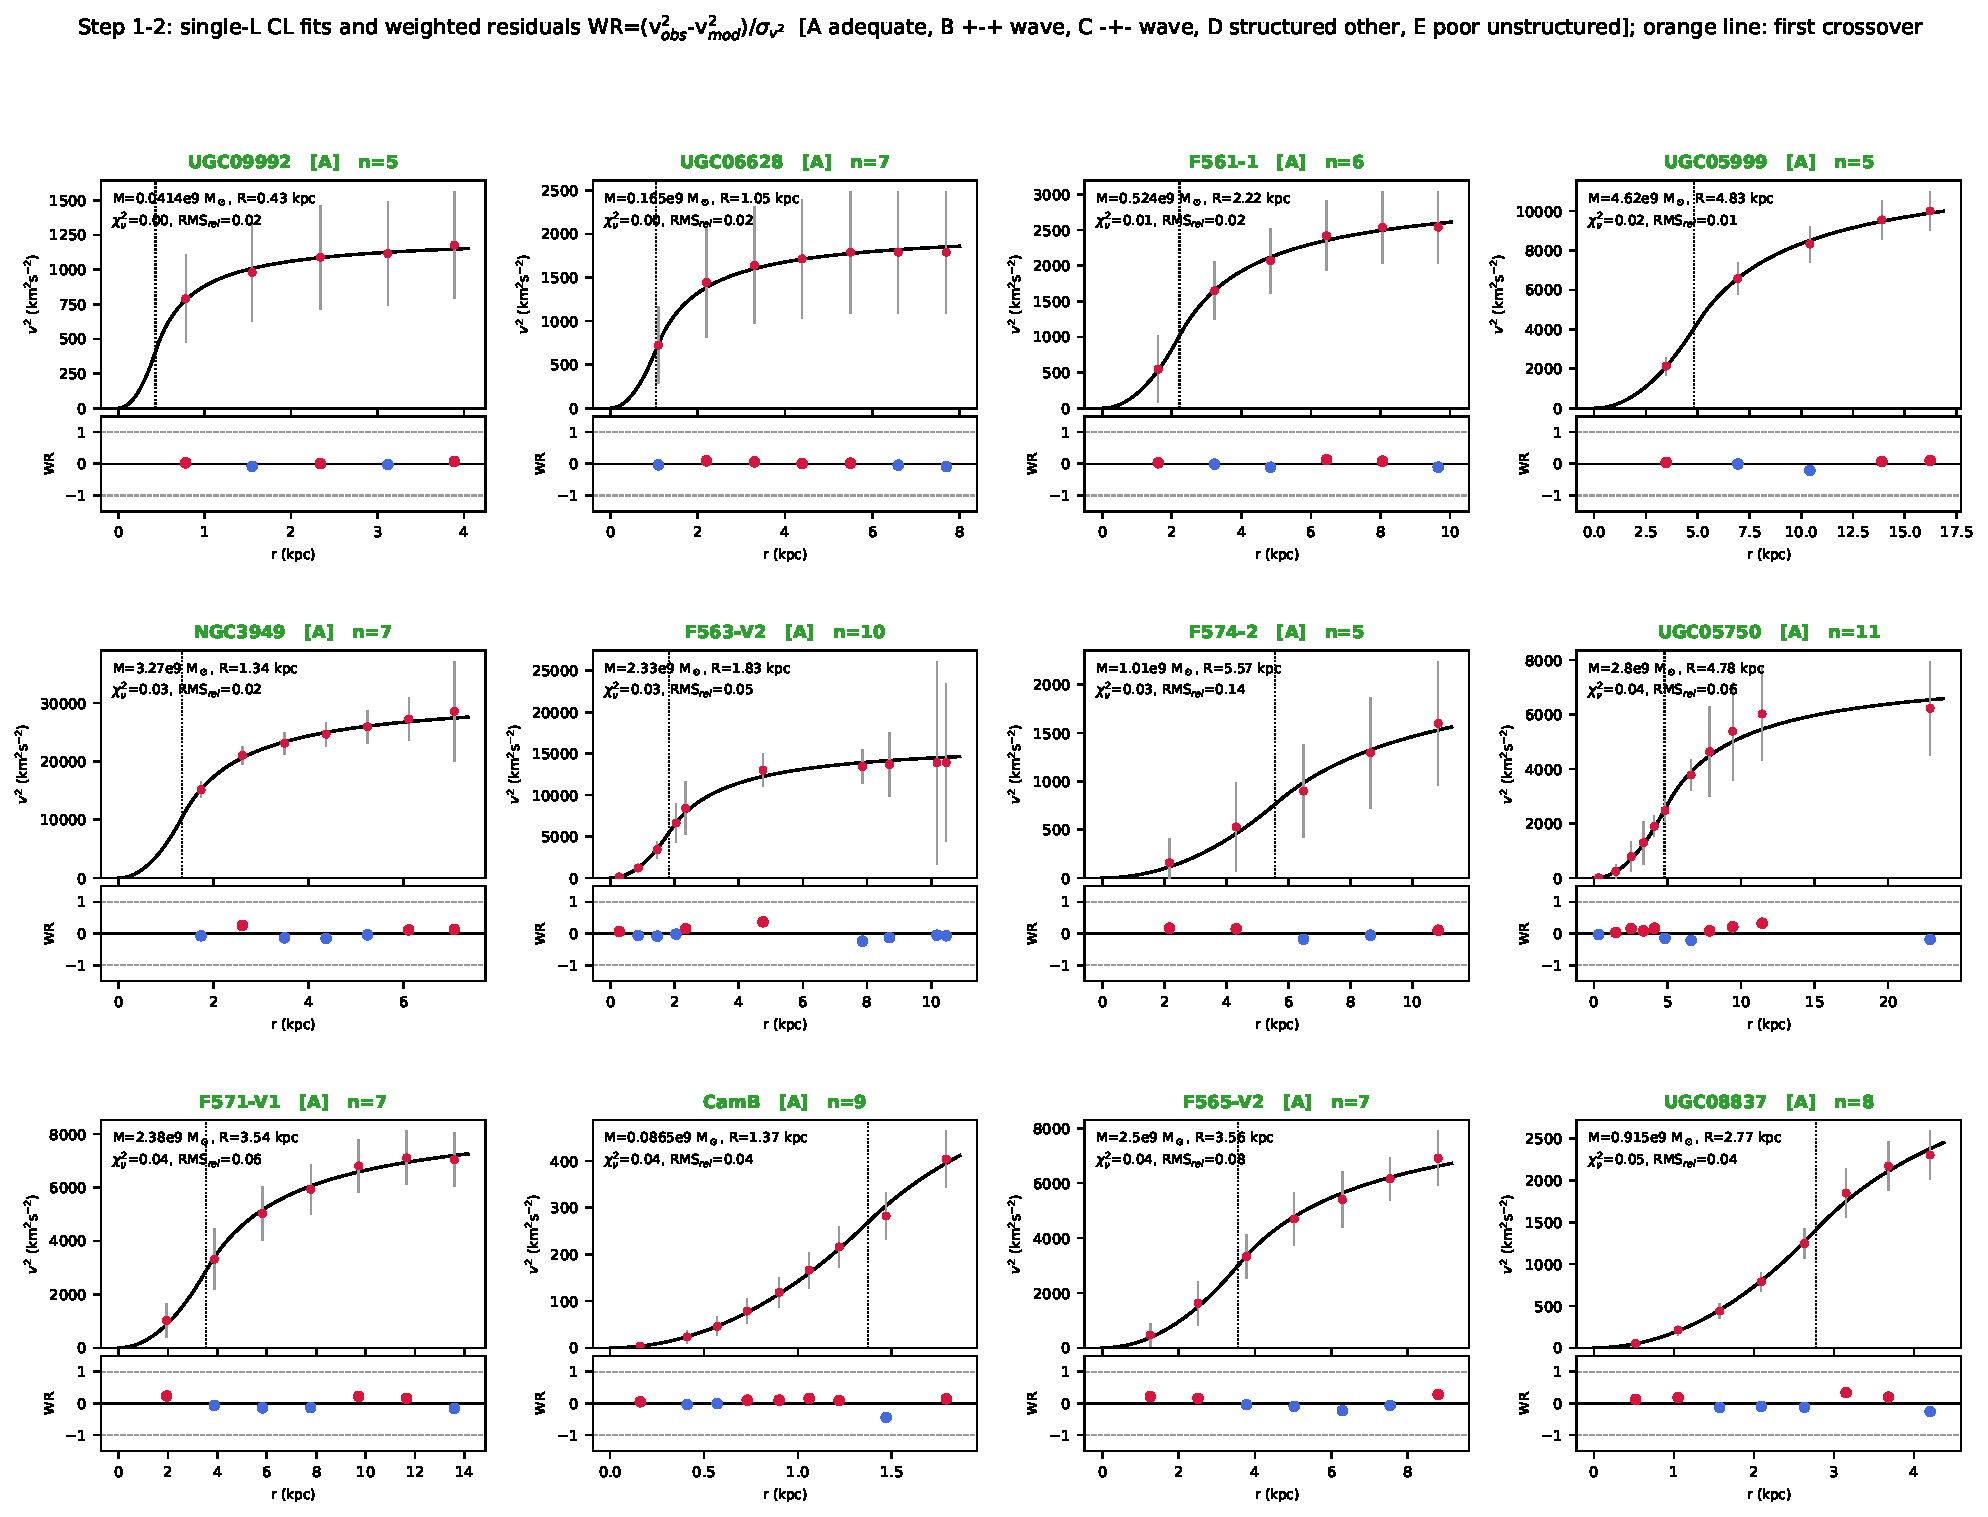
\includepdf[pages=-,fitpaper=false,scale=0.95]{single_L_atlas.pdf}
\section*{Atlas 2: accepted two-L fits with residuals}
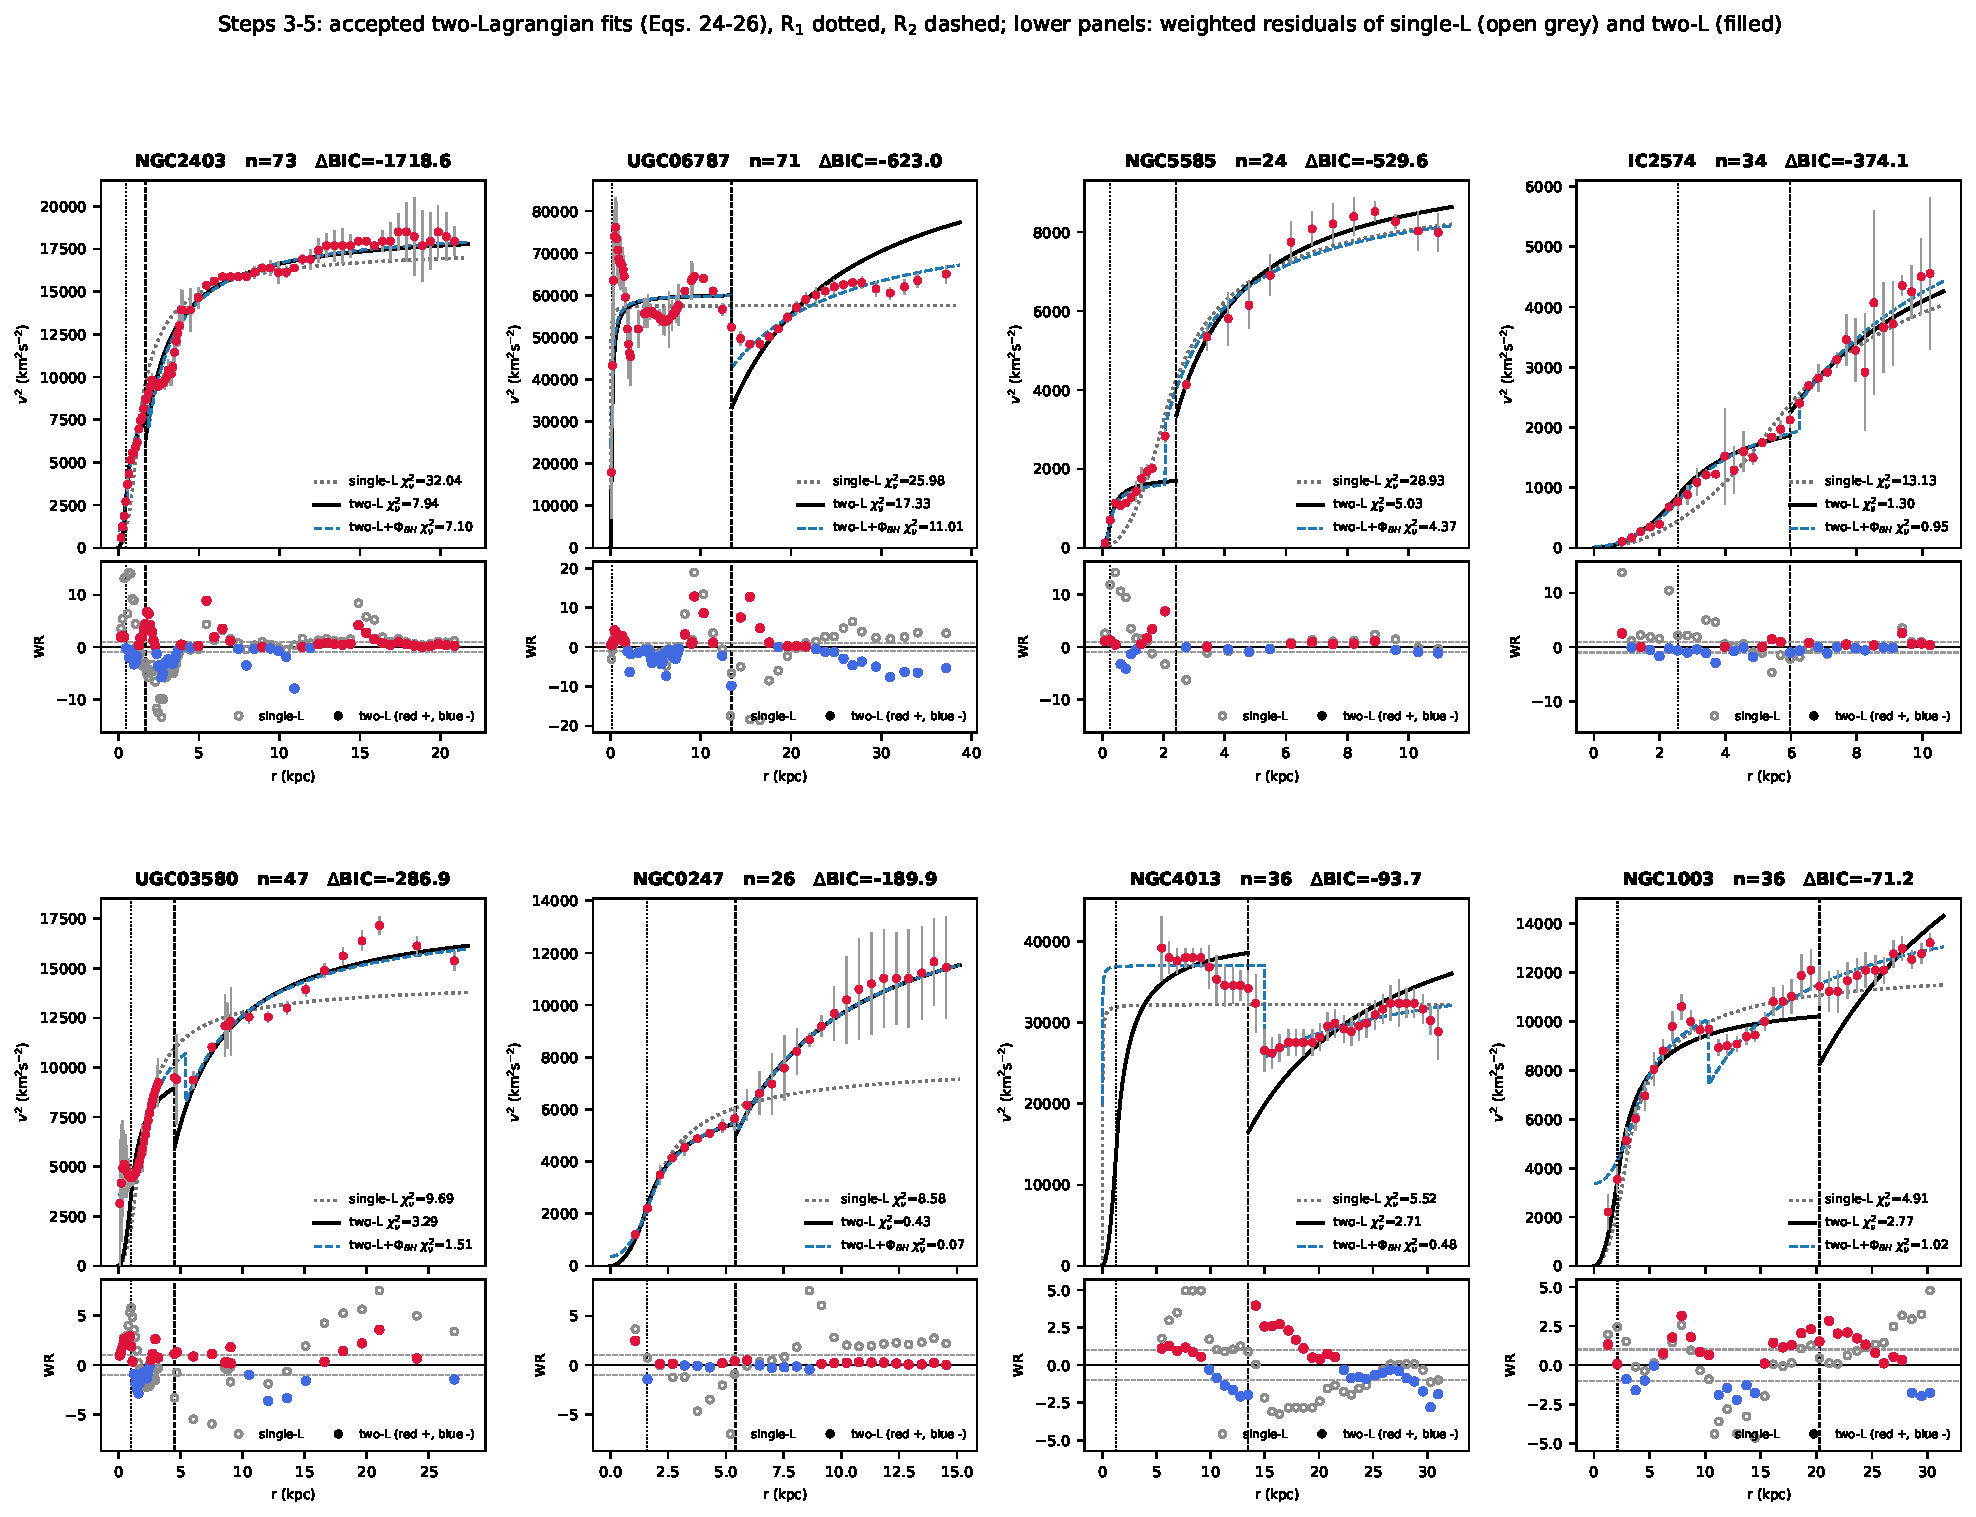
\includepdf[pages=-,scale=0.95]{double_L_atlas.pdf}
\end{document}